\documentclass[border=10pt]{standalone}
\usepackage{pgfplots}
\pgfplotsset{compat=1.18}
\usepgfplotslibrary{fillbetween}
\begin{document}
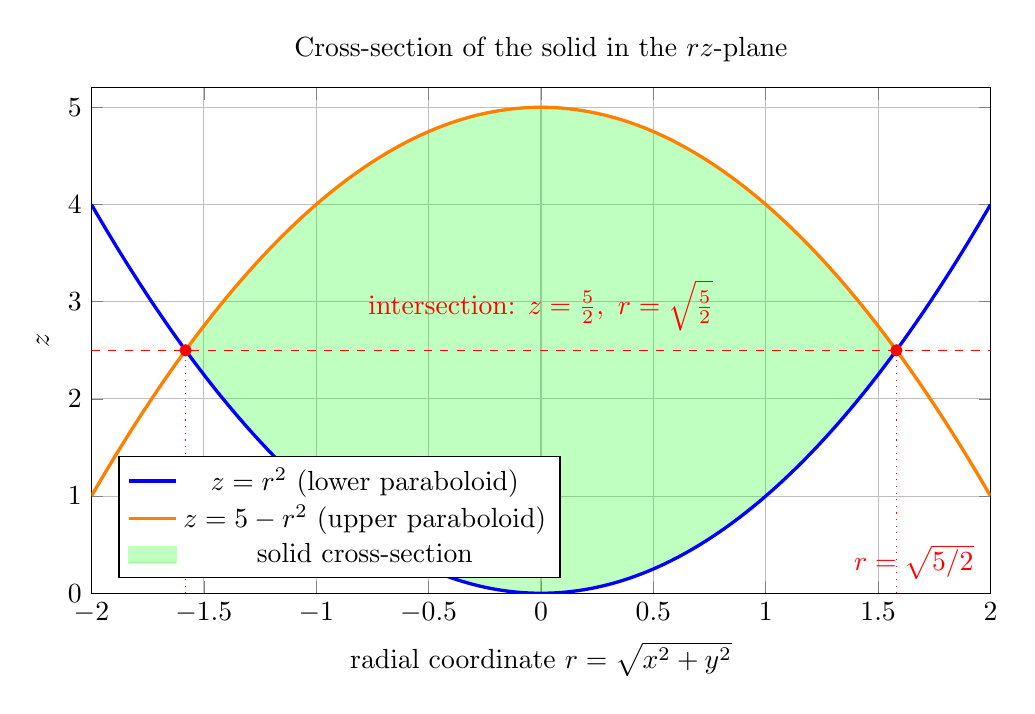
\begin{tikzpicture}
\begin{axis}[
    width=13cm, height=8cm,
    xlabel={radial coordinate $r=\sqrt{x^2+y^2}$},
    ylabel={$z$},
    xmin=-2, xmax=2, ymin=0, ymax=5.2,
    title={Cross-section of the solid in the $rz$-plane},
    legend pos=south west,
    grid=both,
]
\addplot[name path=A, domain=-2:2, samples=200, very thick, blue] {x^2};
\addlegendentry{$z=r^2$ (lower paraboloid)}
\addplot[name path=B, domain=-2:2, samples=200, very thick, orange] {5-x^2};
\addlegendentry{$z=5-r^2$ (upper paraboloid)}
\addplot[green, opacity=0.25] fill between[of=A and B, soft clip={domain=-1.58113883:1.58113883}];
\addlegendentry{solid cross-section}
\draw[dashed, red] (axis cs:-2,2.5) -- (axis cs:2,2.5);
\draw[dotted, red] (axis cs:1.58113883,0) -- (axis cs:1.58113883,2.5);
\draw[dotted, red] (axis cs:-1.58113883,0) -- (axis cs:-1.58113883,2.5);
\addplot[only marks, red, mark=*, mark size=2pt] coordinates {(1.58113883,2.5) (-1.58113883,2.5)};
\node[red, anchor=south] at (axis cs:0,2.6) {intersection: $z=\frac{5}{2},\ r=\sqrt{\frac{5}{2}}$};
\node[red, anchor=west] at (axis cs:1.35,0.32) {$r=\sqrt{5/2}$};
\end{axis}
\end{tikzpicture}
\end{document}
